\chapter{Классификация сетей. Требования к ним}

Для классификации компьютерных сетей используются различные признаки, но чаще всего сети делят на типы \textbf{\textit{по территориальному признаку или масштабу производственного подразделения}}.

\section{Локальные и глобальные сети}

При использовании \textbf{\textit{территориального признака, то есть по величине территории, которую покрывает сеть, они делятся на}}:
\begin{itemize}
    \item локальные сети;
    \item глобальные сети;
    \item городские сети.
\end{itemize}

\subsection{Локальные сети}

К  \textbf{\textit{локальным сетям (Local Area Networks, LAN)}} относятся сети компьютеров, сосредоточенные на небольшой территории (обычно в радиусе не более 1-2 км).
В общем случае локальная сеть представляет собой коммуникационную систему, принадлежащую одной организации.
Из-за коротких расстояний в локальных сетях имеется возможность использовать относительно дорогие высококачественные линии связи, которые позволяют достигать высоких скоростей обмена данными (100 Мбит/с и более). В связи с этим услуги, предоставляемые локальными сетями, отличаются широким разнообразием и обычно предусматривают реализацию в режиме on-line.

\subsection{Глобальные сети}

\textbf{\textit{Глобальные сети (Wide Area Networks, WAN)}} - объединяют территориально рассредоточенные компьютеры, которые могут находиться в различных городах и странах.
В глобальных сетях часто используются уже существующие линии связи, изначально предназначенные совсем для других целей, например, телефонные и телеграфные каналы общего назначения.
Из-за низких скоростей таких линий связи в глобальных сетях (десятки килобит в секунду) набор предоставляемых услуг обычно ограничивается передачей файлов, преимущественно не в оперативном, а в фоновом режиме, с использованием электронной почты.
Для устойчивой передачи дискретных данных по некачественным линиям связи применяются методы и оборудование, существенно отличающиеся от методов и оборудования, характерных для локальных сетей.
Как правило, здесь применяются сложные процедуры контроля и восстановления данных, так как наиболее типичный режим передачи данных по территориальному каналу связи связан со значительными искажениями сигналов.

\subsection{Городские сети}

\textbf{\textit{Городские сети (или сети мегаполисов) - Metropolitan Area Networks (MAN)}} являются менее распространенным типом сетей, они появились сравнительно недавно и предназначены для обслуживания территории крупного города - мегаполиса.
Локальные сети наилучшим образом подходят для разделения ресурсов на коротких расстояниях и широковещательных передач.
Глобальные сети обеспечивают работу на больших расстояниях, но с ограниченной скоростью.
Сети мегаполисов занимают некоторое промежуточное положение.

Они используют цифровые магистральные линии связи, часто оптоволоконные, со скоростями от 45 Мбит/с, и предназначены для связи локальных сетей в масштабах города и соединения локальных сетей с глобальными.

\subsection{Отличия локальных сетей от глобальных}

Рассмотрим основные отличия локальных сетей от глобальных, хотя необходимо заметить, что в последнее время они становятся все менее заметными.
\begin{itemize}
    \item Протяженность, качество и способ прокладки линий связи.
        Класс локальных вычислительных сетей по определению отличается от класса глобальных сетей меньшими расстояниями между узлами сети.
        Это в принципе делает возможным использование в локальных сетях качественных линий связи, которые не всегда доступны (из-за экономических ограничений) на больших расстояниях, свойственных глобальным сетям.
        В глобальных сетях часто применяются уже существующие линии связи (телеграфные или телефонные), а в локальных сетях они прокладываются заново.
    \item Сложность методов передачи и оборудования.
        В условиях низкой надежности физических каналов в глобальных сетях требуются более сложные, чем в локальных сетях, методы передачи данных и соответствующее оборудование.
        Так, в глобальных сетях широко применяются модуляция, асинхронные методы, сложные методы контрольного суммирования, квитирование и повторные передачи искаженных кадров.
        С другой стороны, качественные линии связи в локальных сетях позволили упростить процедуры передачи данных за счет применения немодулированных сигналов и отказа от обязательного подтверждения получения пакета.
    \item Скорость обмена данными.
        Одним из главных отличий локальных сетей от глобальных является наличие высокоскоростных каналов обмена данными между компьютерами, скорость которых (10, 16, 100 Мбит/с и более) сравнима со скоростями работы устройств и узлов компьютера.
        Для глобальных сетей типичны гораздо более низкие скорости передачи данных - 2400, 9600, 28800, 33600 бит/с, 56 и 64 Кбит/с и только на магистральных каналах - до 2 Мбит/с.
    \item Разнообразие предоставляемых  услуг.
        Локальные сети предоставляют, как правило, широкий набор услуг - это различные виды услуг файловой службы, услуги печати, услуги службы передачи факсимильных сообщений, услуги баз данных, электронная почта и другие, в то время как глобальные сети в основном предоставляют почтовые услуги и иногда файловые услуги с ограниченными возможностями.
    \item Оперативность выполнения запросов.
        Время прохождения пакета через локальную сеть обычно составляет несколько миллисекунд, время же его передачи через глобальную сеть может достигать нескольких секунд, что затрудняет реализацию служб для режима on-line.
    \item Разделение каналов.
        В локальных сетях каналы связи используются, как правило, совместно сразу несколькими узлами сети; а в глобальных сетях - индивидуально.
\end{itemize}

\subsection{Тенденция к сближению локальных и глобальных сетей}

Если принять во внимание все перечисленные выше различия локальных и глобальных сетей, то становится понятным, почему так долго могли существовать раздельно два сообщества специалистов, занимающиеся этими двумя видами сетей.
Но за последние годы ситуация резко изменилась.

Специалисты по локальным сетям, перед которыми встали задачи объединения нескольких локальных сетей, расположенных в разных, географически удаленных друг от друга пунктах, были вынуждены начать освоение чуждого для них мира глобальных сетей и телекоммуникаций.

С другой стороны, стремление повысить пропускную способность, скорость передачи данных, расширить набор и оперативность служб, другими словами, стремление улучшить качество предоставляемых услуг - все это заставило специалистов по глобальным сетям обратить пристальное внимание на технологии, используемые в локальных сетях.

Таким образом, в мире локальных и глобальных сетей явно наметилось движение навстречу друг другу, которое уже сегодня привело к значительному взаимопроникновению технологий локальных и глобальных сетей.

\textbf{\textit{Сближение в методах передачи данных}} происходит на платформе оптической цифровой (немодулированной) передачи данных по оптоволоконным линиям связи.
Из-за резкого улучшения качества каналов связи в глобальных сетях начали отказываться от сложных и избыточных процедур обеспечения корректности передачи данных и скорости передачи данных в уже существующих коммерческих глобальных сетях нового поколения приближаются к традиционным скоростям локальных сетей (в сетях Frame Relay сейчас доступны скорости 2 Мбит/с), а в глобальных сетях АТМ и превосходят их, достигая 622 Мбит/с.

В результате службы \textbf{\textit{режима on-line}} становятся обычными и в глобальных сетях.
Наиболее яркий пример - гипертекстовая информационная служба World Wide Web, ставшая основным поставщиком информации в сети Internet.
Ее интерактивные возможности превзошли возможности многих аналогичных служб локальных сетей, так что разработчикам локальных сетей пришлось просто позаимствовать эту службу у глобальных сетей.

\textbf{\textit{Локальные сети перенимают у глобальных сетей и транспортные технологии}}.
Все новые скоростные технологии (Fast Ethernet, Gigabit Ethernet, l00VG-AnyLAN) поддерживают работу по \textbf{\textit{индивидуальным линиям связи наряду}} с традиционными для локальных сетей разделяемыми линиями.
Для организации индивидуальных линий связи используется специальный тип коммуникационного оборудования - коммутаторы.

В локальных сетях в последнее время уделяется такое же большое внимание методам обеспечения \textbf{\textit{защиты информации от несанкционированного доступа}}, как и в глобальных сетях.
Такое внимание обусловлено тем, что локальные сети перестали быть изолированными, чаще всего они имеют выход в «большой мир» через глобальные связи.

И, наконец, появляются \textbf{\textit{новые технологии, изначально предназначенные для обоих видов сетей}}.
Наиболее ярким представителем нового поколения технологий является технология АТМ, которая может служить основой не только локальных и глобальных компьютерных сетей, но и телефонных сетей, а также широковещательных видеосетей, объединяя все существующие типы трафика в одной транспортной сети.

\section{Сети отделов, кампусов и корпораций}

Еще одним популярным способом классификации сетей является их классификация по масштабу производственного подразделения, в пределах которого действует сеть.
Различают:
\begin{itemize}
    \item сети отделов;
    \item сети кампусов;
    \item корпоративные сети.
\end{itemize}

\subsection{Сети отделов}

\textbf{\textit{Сети отделов}} - это сети, которые используются сравнительно небольшой группой сотрудников, решающих общие задачи и работающих в одном отделе предприятия.
Считается, что отдел может насчитывать до 100 - 150  сотрудников.

Главной целью сети отдела является \emph{разделение локальных ресурсов}, таких как приложения, данные, лазерные принтеры и модемы.
Обычно сети отделов имеют один или два файловых сервера и не более тридцати пользователей (рисунок).
Сети отделов обычно не разделяются на подсети.
В этих сетях локализуется большая часть трафика предприятия.
Сети отделов обычно создаются на основе какой-либо одной сетевой технологии - Ethernet, Token Ring.
\begin{figure}[!ht]
    \centering
    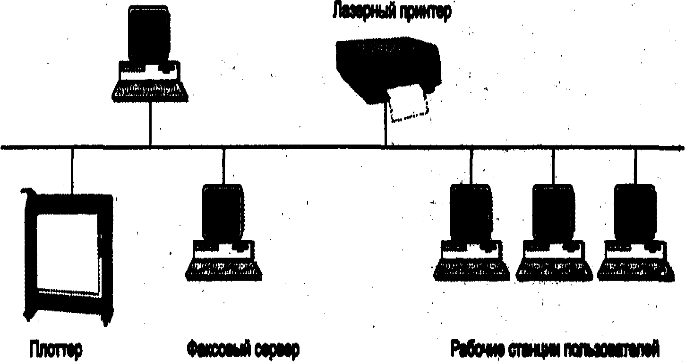
\includegraphics[width=0.7\textwidth]{department-network-example}
    \caption{Пример сети масштаба отдела}
    \label{fig:department-network-example}
\end{figure}

Задачи управления сетью на уровне отдела относительно просты: добавление новых пользователей, устранение простых отказов, инсталляция новых узлов и установка новых версий программного обеспечения.
Такой сетью может управлять сотрудник, не имеющий специальной подготовки.

\subsection{Сети кампусов}

\textbf{\textit{Сети кампусов}} получили свое название от английского слова campus - студенческий городок, где часто возникала необходимость объединения нескольких мелких сетей в одну большую сеть.

Главными особенностями сетей кампусов (рис.) являются следующие:
\begin{itemize}
    \item Сети этого типа объединяют множество сетей различных отделов одного предприятия в пределах отдельного здания или в пределах одной территории, покрывающей площадь в несколько квадратных километров.
    \item Глобальные соединения в сетях кампусов не используются.
    \item Службы такой сети включают взаимодействие между сетями отделов, доступ к общим базам данных предприятия, доступ к общим факс-серверам, высокоскоростным модемам и высокоскоростным принтерам.
        В результате сотрудники каждого отдела предприятия получают доступ к некоторым ресурсам сетей других отделов.
    \item Важной службой, предоставляемой сетями кампусов, стал доступ к корпоративным базам данных независимо от того, на каких типах компьютеров они располагаются.
\end{itemize}

Именно на уровне сети кампуса возникают проблемы интеграции неоднородного аппаратного и программного обеспечения.
Типы компьютеров, сетевых операционных систем, сетевого аппаратного обеспечения могут отличаться в каждом отделе.
Отсюда вытекают сложности управления сетями кампусов.
Администраторы должны быть в этом случае более квалифицированными, а средства оперативного управления сетью - более совершенными.

\begin{figure}
    \centering
    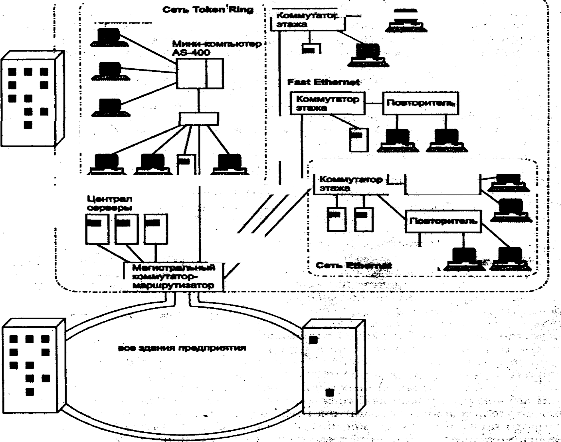
\includegraphics[width=0.7\textwidth]{campus-network-example}
    \caption{Пример сети кампуса}
    \label{fig:campus-network-example}
\end{figure}

\subsection{Корпоративные сети}

\textbf{\textit{Корпоративные сети}} называют также сетями масштаба предприятия, они объединяют большое количество компьютеров на всех территориях отдельного предприятия.
Они могут быть сложно связаны и покрывать город, регион или даже континент.
Число пользователей и компьютеров может измеряться тысячами, а число серверов - сотнями, расстояния между сетями отдельных территорий могут оказаться такими, что становится необходимым использование глобальных связей (рисунок).

Непременным \textbf{\textit{атрибутом}} такой сложной и крупномасштабной сети обязательно будет \textbf{\textit{гетерогенность}} - использование различных типов компьютеров, операционных систем и множества различных приложений.

\begin{figure}
    \centering
    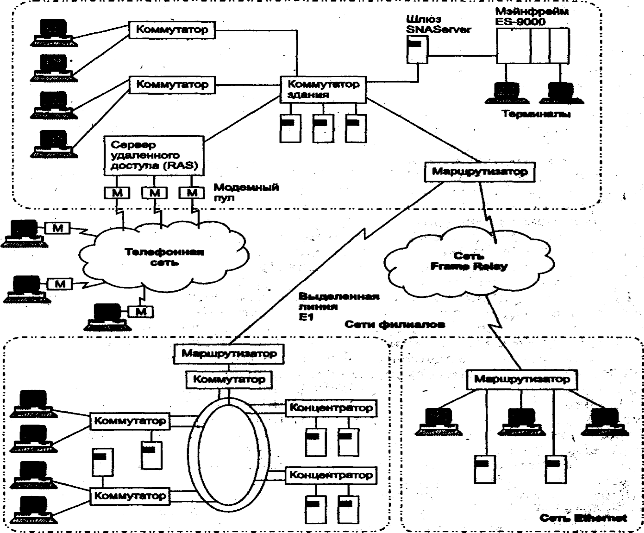
\includegraphics[width=0.7\textwidth]{corporate-network-example}
    \caption{Пример корпоративной сети}
    \label{fig:corporate-network-example}
\end{figure}

\section{Требования, предъявляемые к современным  вычислительным сетям}

Главным требованием, предъявляемым к сетям, является \emph{выполнение сетью ее основной функции - обеспечение пользователям потенциальной возможности доступа к разделяемым ресурсам всех компьютеров, объединенных в сеть}.
Все остальные требования - производительность, надежность, совместимость, управляемость, защищенность, расширяемость и масштабируемость - связаны с качеством выполнения этой основной задачи.

Хотя все эти требования весьма важны, часто понятие \textbf{\textit{«качество обслуживания» (Quality of Service, QoS)}} компьютерной сети трактуется более узко - в него включаются только две самые важные характеристики сети – \textbf{\textit{производительность и надежность.}}

Независимо от выбранного показателя качества обслуживания сети существуют \textbf{\textit{два подхода к обеспечению качества обслуживания}}.

\emph{Первый подход} состоит в том, что сеть (точнее, обслуживающий ее персонал) гарантирует пользователю соблюдение некоторой числовой величины показателя качества обслуживания.
Например, сеть может гарантировать пользователю А, что любой из его пакетов, посланных пользователю В, будет задержан сетью не более, чем на 150 мс.
Или, что средняя пропускная способность канала между пользователями А и В не будет ниже 5 Мбит/с, при этом канал будет разрешать пульсации трафика в 10 Мбит на интервалах времени не более 2 секунд.
Технологии Frame Relay и АТМ позволяют строить сети, гарантирующие качество обслуживания по производительности.

\emph{Второй подход} состоит в том, что сеть обслуживает пользователей в соответствии с их приоритетами.
То есть качество обслуживания зависит от степени привилегированности пользователя или группы пользователей, к которой он принадлежит.
Качество обслуживания в этом случае не гарантируется, а гарантируется только уровень привилегий пользователя.
Такое обслуживание называется обслуживанием best effort - с наибольшим старанием.

\subsection{Производительность}
Потенциально высокая \textbf{\textit{производительность}} - это одно из основных свойств распределенных систем, к которым относятся компьютерные сети.
Это свойство обеспечивается возможностью распараллеливания работ между несколькими компьютерами сети.
К сожалению, эту возможность не всегда удается реализовать.
Существует несколько основных характеристик \textbf{\textit{производительности сети}}:
\begin{itemize}
    \item \emph{время реакции};
    \item \emph{пропускная способность};
    \item \emph{задержка передачи и вариация задержки передачи}.
\end{itemize}

\textbf{\textit{Время реакции}} сети является интегральной характеристикой производительности сети с точки зрения пользователя.
Именно эту характеристику имеет в виду пользователь, когда говорит: «Сегодня сеть работает медленно».

В общем случае \emph{время реакции определяется как интервал времени между возникновением запроса пользователя к какой-либо сетевой службе и получением ответа на этот запрос}.

Очевидно, что значение этого показателя зависит от различных факторов, поэтому имеет смысл использовать средневзвешенную оценку времени реакции сети, усредняя этот показатель по пользователям, серверам и времени дня.

\textbf{\textit{Пропускная способность}} отражает объем данных, переданных сетью или ее частью в единицу времени.
Пропускная способность уже не является пользовательской характеристикой, так как она говорит о скорости выполнения внутренних операций сети - передачи пакетов данных между узлами сети через различные коммуникационные устройства.
Зато она непосредственно характеризует качество выполнения основной функции сети - транспортировки сообщений - и поэтому чаще используется при анализе производительности сети, чем время реакции.

Пропускная способность измеряется либо в битах в секунду, либо в пакетах в секунду.
Пропускная способность может быть:
\begin{itemize}
    \item мгновенной;
    \item максимальной;
    \item средней.
\end{itemize}

\emph{Средняя пропускная способность вычисляется путем деления общего объема переданных данных на время их передачи, причем выбирается достаточно длительный промежуток времени - час, день или неделя.}

\emph{Мгновенная пропускная способность отличается от средней тем, что для усреднения выбирается очень маленький промежуток времени - например, 10 мс или 1 с.}

\emph{Максимальная пропускная способность - это наибольшая мгновенная пропускная способность, зафиксированная в течение периода наблюдения.}

Чаще всего при проектировании, настройке и оптимизации сети используются такие показатели, как средняя и максимальная пропускные способности.
Средняя пропускная способность отдельного элемента или всей сети позволяет оценить работу сети на большом промежутке времени, в течение которого в силу закона больших чисел пики и спады интенсивности трафика компенсируют друг друга.
Максимальная пропускная способность позволяет оценить возможности сети справляться с пиковыми нагрузками, характерными для особых периодов работы сети, например утренних часов, когда сотрудники предприятия почти одновременно регистрируются в сети и обращаются к разделяемым файлам и базам данных.

\textbf{\textit{Задержка передачи}} определяется как промежуток времени между моментом поступления пакета на вход какого-либо сетевого устройства или части сети и моментом появления его на выходе этого устройства.
Этот параметр производительности по смыслу близок ко времени реакции сети, но отличается тем, что всегда характеризует только сетевые этапы обработки данных, без задержек обработки компьютерами сети.

Обычно качество сети характеризуют величинами \emph{максимальной задержки передачи и вариацией задержки}.
Не все типы трафика чувствительны к задержкам передачи.
Так задержки пакетов, порождаемых файловой службой, службой электронной почты или службой печати, мало влияют на качество этих служб с точки зрения пользователя сети.
С другой стороны, такие же задержки пакетов, переносящих голосовые данные или видеоизображение, могут приводить к значительному снижению качества предоставляемой пользователю информации - возникновению эффекта «эха», невозможности разобрать некоторые слова, дрожанию изображения и т.
п.

\textbf{\textit{Внимание! Пропускная способность и задержка передачи являются независимыми параметрами, так что сеть может обладать, например, высокой пропускной и, при этом, вносить значительные задержки при передаче каждого пакета.}}
Пример такой ситуации дает канал связи, образованный геостационарным спутником.
Пропускная способность этого канала может быть весьма высокой, например 2 Мбит/с то время как задержка передачи всегда составляет не менее 0,24 с, что определяется скоростью распространения сигнала (около 300 000 км/с) и длиной канала (72 000 км).

\subsection{Надежность и безопасность}
Одной из первоначальных целей создания распределенных систем, к которым относятся и вычислительные сети, являлось достижение большей надежности по сравнению с отдельными вычислительными машинами.

Важно различать несколько аспектов \textbf{\textit{надежности}}.
Применяемые для технических устройств такие показатели надежности, как среднее время наработки на отказ, вероятность отказа, интенсивность отказов пригодны для оценки надежности только простых элементов и устройств, которые могут находиться только в двух состояниях - работоспособном или неработоспособном.
Сложные системы кроме состояний работоспособности и неработоспособности, могут иметь и другие промежуточные состояния, в связи с чем для оценки надежности сложных систем применяется другой набор характеристик.

\emph{Готовность или коэффициент готовности (availability)} означает долю времени, в течение которого система может быть использована.
Готовность может быть улучшена путем введения избыточности в структуру системы: ключевые элементы системы должны существовать в нескольких экземплярах, чтобы при отказе одного из них функционирование системы обеспечивали другие.

Кроме того система должна обеспечить \emph{сохранность данных и защиту их от искажений}.

Так как сеть работает на основе механизма передачи пакетов между конечными узлами, то одной из характерных характеристик надежности является \emph{вероятность доставки пакета узлу назначения без искажений}.
Наряду с этой характеристикой могут использоваться и другие показатели: \emph{вероятность потери пакета, вероятность искажения отдельного бита передаваемых данных, отношение числа потерянных пакетов к доставленным}.

Другим аспектом общей надежности является \textbf{\textit{безопасность (security)}}, то есть способность системы защитить данные от несанкционированного доступа.
В распределенной системе это сделать гораздо сложнее, чем в централизованной.

Еще одной характеристикой надежности является \emph{отказоустойчивость (fault tolerance)}.
В сетях под отказоустойчивостью понимается способность системы скрыть от пользователя отказ отдельных ее элементов.
Например, если копии таблицы базы данных хранятся одновременно на нескольких файловых серверах, то пользователи могут просто не заметить отказ одного из них.
В отказоустойчивой системе отказ одного из ее элементов приводит к некоторому снижению качества ее работы (деградации), а не к полному останову.

Расширяемость и масштабируемость
Термины \emph{расширяемость} и \emph{масштабируемость} иногда используют как синонимы, но это неверно - каждый из них имеет четко определенное самостоятельное значение.

\emph{Расширяемость (extensibility)} означает возможность сравнительно легкого добавления отдельных элементов сети (пользователей, компьютеров, приложений, служб), наращивания длины сегментов сети и замены существующей аппаратуры более мощной.
При этом принципиально важно, что легкость расширения системы иногда может обеспечиваться в некоторых весьма ограниченных пределах.
Например, локальная сеть Ethernet, построенная на основе одного сегмента толстого коаксиального кабеля, обладает хорошей расширяемостью, в том смысле, что позволяет легко подключать новые станции.
Однако такая сеть имеет ограничение на число станций - их число не должно превышать 30-40.
Хотя сеть допускает физическое подключение к сегменту и большего числа станций (до 100), но при этом чаще всего резко снижается производительность сети.
Наличие такого ограничения и является признаком плохой масштабируемости системы при хорошей расширяемости.

\emph{Масштабируемость (scalability)} означает, что сеть позволяет наращивать количество узлов и протяженность связей в очень широких пределах, при этом производительность сети не ухудшается.
Для обеспечения масштабируемости сети приходится применять дополнительное коммуникационное оборудование и специальным образом структурировать сеть.
Например, хорошей масштабируемостыо обладает многосегментная сеть, построенная с использованием коммутаторов и маршрутизаторов и имеющая иерархическую структуру связей.
Такая сеть может включать несколько тысяч компьютеров и при этом обеспечивать каждому пользователю сети нужное качество обслуживания.

\subsection{Прозрачность}
\emph{Прозрачность (transparency)} сети достигается в том случае, когда сеть представляется пользователям не как множество отдельных компьютеров, связанных между собой сложной системой кабелей, а как единая традиционная вычислительная машина с системой разделения времени.
Известный лозунг компании Sun MicroeyftemK «Сеть - это компьютер» - говорит именно о такой прозрачной сети.

Прозрачность может быть достигнута на двух различных уровнях - на уровне пользователя и на уровне программиста.
На уровне пользователя прозрачность означает, что для работы с удаленными ресурсами он использует те же команды и привычные ему процедуры, что и для работы с локальными ресурсами.
На программном уровне прозрачность заключается в том, что приложению для доступа к удаленным ресурсам требуются те же вызовы, что и для доступа к локальным ресурсам.
Прозрачность на уровне пользователя достигается проще, так как все особенности процедур, связанные с распределенным характером системы, маскируются от пользователя программистом, который создает приложение.
Прозрачность на уровне приложения требует сокрытия всех деталей распределенности средствами сетевой операционной системы.

\subsection{Поддержка разных видов трафика}
Компьютерные сети изначально предназначены для совместного доступа пользователя к ресурсам компьютеров: файлам, принтерам и т.
п.
Однако 90-е годы стали годами проникновения в компьютерные сети трафика мультимедийных данных, представляющих в цифровой форме речь и видеоизображение.
Естественно, что \textbf{\textit{для динамической передачи мультимедийного трафика требуются иные алгоритмы и протоколы}} и, соответственно, другое оборудование.

\textbf{\textit{Главной особенностью трафика, образующегося ври динамической передаче голоса или изображения, является наличие жестких требований к синхронности передаваемых сообщений.}}
Для качественного воспроизведения непрерывных процессов, которыми являются звуковые колебания или изменения интенсивности света в видеоизображении, необходимо получение измеренных и закодированных амплитуд сигналов с той же частотой, с которой они были измерены на передающей стороне.
При запаздывании сообщений будут наблюдаться искажения.

В то же время \emph{трафик компьютерных данных характеризуется крайне неравномерной интенсивностью поступления сообщений в сеть при отсутствии жестких требований к синхронности доставки этих сообщений}.
Например, доступ пользователя, работающего с текстом на удаленном диске, порождает случайный поток сообщений между удаленным и локальным компьютерами, зависящий от действий пользователя по редактированию текста.
Отметим, что задержки при доставке в определенных (и достаточно широких с компьютерной точки зрения) пределах такого трафика мало влияют на качество обслуживания пользователя сети.

\emph{Особую сложность представляет совмещение в одной сети традиционного компьютерного и мультимедийного трофика.}

\subsection{Управляемость}
\emph{Управляемость} сети подразумевает возможность централизованно контролировать состояние основных элементов сети, выявлять и разрешать проблемы, возникающие при работе сети, выполнять анализ производительности и планировать развитие сети.
В идеале средства управления сетями представляют собой систему, осуществляющую наблюдение, контроль и управление каждым элементом сети - от простейших до самых сложных устройств, при этом такая система рассматривает сеть как единое целое, а не как разрозненный набор отдельных устройств.

\subsection{Совместимость}
\emph{Совместимость или интегрируемость} означает, что сеть способна включать в себя самое разнообразное программное и аппаратное обеспечение, то есть в ней могут сосуществовать различные операционные системы, поддерживающие разные стеки коммуникационных протоколов, и работать аппаратные средства и приложения от разных производителей.
Сеть, состоящая из разнотипных элементов, называется \emph{неоднородной или гетерогенной}, а если гетерогенная сеть работает без проблем, то она является интегрированной.
Основной путь построения интегрированных сетей - использование модулей, выполненных в соответствии с открытыми стандартами и спецификациями.
